\section{Bildverarbeitung}
\label{anhang-bildverarbeitung}
Die Bildverarbeitung wurde auf Basis von Java und Python geprüft. In beiden Programmiersprachen gibt es viele Bibliotheken, welche Bildoperationen unterstützen. Es beginnt bei einfachen Funktionen wie das Zuschneiden oder Komprimieren von Bildern bis hin über integrierte Objekterkennung.

\subsection{Java}
In Java wurde die Bibliothek ImageJ\footnote{\href{http://imagejdocu.tudor.lu/}{http://imagejdocu.tudor.lu/}} angeschaut. ImageJ ist modular aufgebaut und lässt sich sowohl Nutzen als auch Erweitern. Zweiteres macht die Bibliothek attraktiv, denn es gibt bereits einige Erweiterungen im Netz. Eine solche Erweiterung nennt sich FeatureFinder\footnote{\href{http://imagejdocu.tudor.lu/doku.php?id=plugin:analysis:feature_finder:start}{http://imagejdocu.tudor.lu/doku.php}}. Diese Erweiterung verlangt als Input das zu suchende Objekt und das Bild auf welchem das Objekt gefunden werden muss. In folgendem Beispiel wird gezeigt wie einfach sich ein Bild zuschneiden lässt.

\begin{lstlisting}[caption={Bild zuschneiden mit ImageJ}]
public void crop(ImagePlus imp, int targetWidth, int targetHeight) {
	ImageProcessor ip = imp.getProcessor();
	int cropX = ip.getWidth() / 2;
	int cropY = ip.getHeight() / 2;
	ip.setRoi(cropX, cropY, targetWidth, targetHeight);
	ip = ip.crop();
	BufferedImage croppedImage = ip.getBufferedImage();
	ImageIO.write(croppedImage, "jpg", new File("cropped.jpg"));
}
\end{lstlisting}

Es ist auch möglich das Bild, auf welchem der Korb zu suchen ist, mit eigenen Low-Level Bildverarbeitung Operationen zu verarbeiten. Beispielsweise kann von links nach rechts die Pixel untersucht wurden. Dort wo der Korb steht weisen die einzelnen Pixel eine anderen Charakteristika auf. Auch das Auslesen eines Pixels auf dem Bild ist simpel.

\begin{lstlisting}[caption={Auslesen eines Pixels mit ImageJ}]
private void readSomePixel() {
	ImagePlus im = new ImagePlus("C:/tmp/ALLUSB/Bilder/Scannen0001.jpg");
	ImageProcessor imp = im.getProcessor();

	int[] rgb = new int[3];
	imp.getPixel(5, 5, rgb);
	System.out.println(Arrays.toString(rgb));
}
\end{lstlisting}

\subsection{Python}

Soll das Bild direkt auf dem Raspberry Pi verarbeitet werden, wird Python als Programmiersprache verwendet. Diese Sprache ist schnell zu erlernen und bringt auch alle notwendigen Funktionen mit. Zudem wird Python vom Raspberry Pi optimal unterstützt.

Um Bilder mit Python zu bearbeiten wird die Python Image Library\footnote{\href{http://effbot.org/imagingbook/overview.htm}{http://effbot.org/imagingbook/overview.htm}} verwendet. Die Bibliothek ist ein Bestandteil der Programmiersprache und kann ohne zusätzliche Installationen verwendet werden. Die Python Image Library bietet alle Funktionen die von einer modernen Bildbearbeitungsbibliothek erwartet werden. Sie bietet auch diverse Filter an und die Pixel eines Bildes lassen sich einzeln bearbeiten. 

Für eine erweiterte Objekterkennung wird OpenCV\footnote{\href{http://docs.opencv.org/trunk/doc/py_tutorials/py_tutorials.html}{http://docs.opencv.org/trunk/doc/py\_tutorials/py\_tutorials.html}} unterstützt. OpenCV ist eine Sammlung von Bildalgorithmen mit denen praktisch jegliche Anwendung von einfachen Objekterkennungen bis hin zu maschinellem Lernen möglich ist. Mithilfe von OpenCV kann man so eine Gesichtserkennung mit wenigen Codezeile realisieren.

\begin{lstlisting}[caption={Gesichtserkennung mit OpenCV}]
	import numpy as np
	import cv2
	
	face_cascade = cv2.CascadeClassifier('haarcascade_face.xml')
	eye_cascade = cv2.CascadeClassifier('haarcascade_eye.xml')
	
	img = cv2.imread('sachin.jpg')
	gray = cv2.cvtColor(img, cv2.COLOR_BGR2GRAY)
	faces = face_cascade.detectMultiScale(gray, 1.3, 5)
	for (x,y,w,h) in faces:
	cv2.rectangle(img,(x,y),(x+w,y+h),(255,0,0),2)
	roi_gray = gray[y:y+h, x:x+w]
	roi_color = img[y:y+h, x:x+w]
	eyes = eye_cascade.detectMultiScale(roi_gray)
	for (ex,ey,ew,eh) in eyes:
	cv2.rectangle(roi_color,(ex,ey),(ex+ew,ey+eh),(0,255,0),2)
	
	cv2.imshow('img',img)
	cv2.waitKey(0)
	cv2.destroyAllWindows()
\end{lstlisting}

\begin{figure}[h!]
\centering
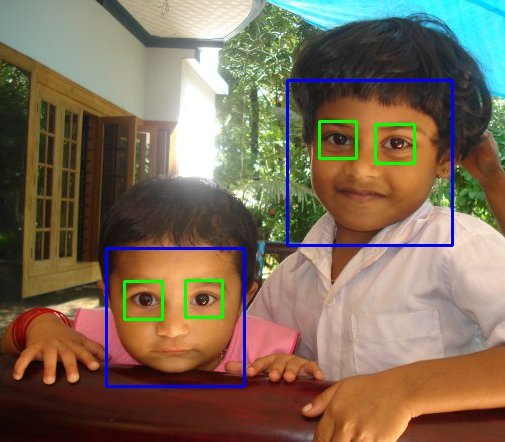
\includegraphics[width=0.7\linewidth]{../../fig/opencv_face}
\caption{Das Ergebnis der Gesichtserkennung}
\label{fig:opencv_face}
\end{figure}
